% This is a sample document using the University of Minnesota, Morris, Computer Science
% Senior Seminar modification of the ACM sig-alternate style. Much of this content is taken
% directly from the ACM sample document illustrating the use of the sig-alternate class. Certain
% parts that we never use have been removed to simplify the example, and a few additional
% components have been added.

% See https://github.com/UMM-CSci/Senior_seminar_templates for more info and to make
% suggestions and corrections.

\documentclass{sig-alternate}
\usepackage{color}
\usepackage{graphicx}
\usepackage{mathtools}
%\usepackage[colorinlistoftodos]{todonotes}

%%%%% Uncomment the following line and comment out the previous one
%%%%% to remove all comments
%%%%%\newcommand{\comment}[1]{}
\newcommand{\comment}[1]{{\bf \tt  {#1}}}
%%%%% NOTE: comments still occupy a line even if invisible;
%%%%% Don't write them as a separate paragraph
\newcommand{\todo}[1]{\textcolor{magenta}{\comment{Todo: {#1}}}}

\begin{document}

% --- Author Metadata here ---
%%% REMEMBER TO CHANGE THE SEMESTER AND YEAR
\conferenceinfo{UMM CSci Senior Seminar Conference, May 2015}{Morris, MN}

\title{Monte Carlo Tree Search and Its Applications}

\numberofauthors{1}

\author{
% The command \alignauthor (no curly braces needed) should
% precede each author name, affiliation/snail-mail address and
% e-mail address. Additionally, tag each line of
% affiliation/address with \affaddr, and tag the
% e-mail address with \email.
\alignauthor
Max Magnuson\\
	\affaddr{Division of Science and Mathematics}\\
	\affaddr{University of Minnesota, Morris}\\
	\affaddr{Morris, Minnesota, USA 56267}\\
	\email{magnu401@morris.umn.edu}
}

\maketitle
\begin{abstract}

\end{abstract}

\keywords{Monte Carlo Tree Search, Heuristics, Upper Confidence Bounds, Artificial Intelligence}

\section{Introduction} 
In 1997 the field of artificial intelligence(AI) experienced a monumental breakthrough when IBM's Deep Blue defeated Garry Kasparov, a reigning grand master, in a chess match\cite{TheGrandChallenge}. The researchers were able to achieve this by using brute force deterministic tree searching methods combined with human knowledge of chess. The human knowledge allows the AI to evaluate the strategic value of a move much like a grand master would, and then populate a tree to search for the best move. This event demonstrated to the world the power of computers and artificial intelligence. 

While computers are capable of outplaying the top players of chess, they struggle when it comes to board games like Go\cite{TheGrandChallenge}. Go is a board game about positional board advantage which is something traditional AI struggles with. They struggle because moves in Go tend to have very long dependencies. A single move may have major effects on moves 50 to 100 moves ahead\cite{RAVEinGo}. This makes game trees for Go significantly deeper than chess. Go also has many more moves available to the player at anyone time than chess. This makes the game trees for Go much wider than in chess. These problems cause deterministic approaches to perform poorly. It is just too much for those approaches to efficiently handle.

People have started turning to alternative methods to approach Go. One such method, Monte Carlo tree search(MCTS), has had a lot of success in Go. MCTS eschews the typical brute force tree searching methods, and it utilizes statistical processes and heuristic approaches to decide what move to make. In 2009, for the first time ever, a computer defeated a top professional Go player in a 9x9 game\cite{TheGrandChallenge}. It took twelve years for AI to advance from defeating Garry Kasparov to achieve its first major victory in Go, and it was only on the smallest board that Go is played on.

MCTS has been growing in popularity in recent years, and it demonstrates a lot of promise. In this paper we will be examining MCTS and a few of its applications.  
\section{Background}
MCTS combines the random sampling of traditional Monte Carlo methods with tree searching. Monte Carlo methods use repeated random sampling to obtain results. The random sampling is used to construct a game tree. This tree will be traversed based on statistical processes, and the MCTS method relies on the convergence of the traversal to reliably choose the best move. The traversal is in convergence when the traversal selects the same path on each traversal. MCTS is a heuristic method and as such it will not always find the most optimal move, but it has a reasonably high success of choosing moves that will lead to greater chances of winning.
\subsection{The Tree Structure}
MCTS structures the game state and its potential moves in a tree. Each node in the tree represents the state of the game with the root node representing the current state. Each line represents a legal move that can be made from one game state to another. In other words, it represents the transformation from the parent node to the child node. Any node may have as many children as there are legal moves. For example, at the start of a game of Tic-Tac-Toe the root node may have up to nine children, one for each possible move. Each following child can only have one less child than its parent since the previous moves are no longer available as options.

\begin{figure}[h]
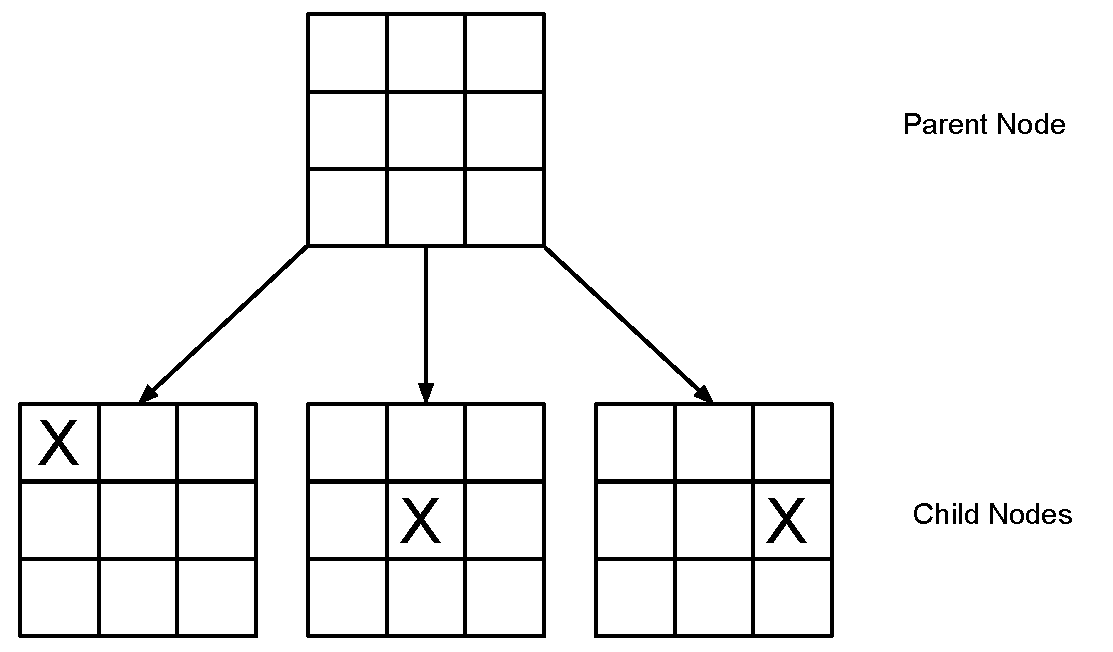
\includegraphics[width=8cm]{TicTacToeTree.pdf}
\centering
\caption{A small portion of what a tree for TicTacToe represents}
\label{fig:TicTacToe}
\end{figure}

Figure \ref{fig:TicTacToe} represents the top portion of a tree for the game Tic-Tac-Toe. The AI is making the first move, so the source node is the first game board. Each child node represents the potential moves that can be made from the current game state. It is important to note here that those are only three of the potential nine child nodes. In the naive implementation of MCTS, each potential child node must be added to the tree before any of those child nodes can be traversed. Other variations of the MCTS algorithm have ways of avoiding this requirement\cite{ActionSelection}. Once MCTS has decided which move to make, the source node of the tree will then become the child it chose. For example, if MCTS chose the left child in figure \ref{fig:TicTacToe}, then the new MCTS tree would start at that child and discard every other child node. 

Along with the game state, each node contains a value that gives an estimate of wins compared to total games in that subtree. The higher the value, the greater proportion of wins in that subtree. The lower the value, the smaller the proportion of wins in that subtree. By choosing the node with the greatest estimated value, the MCTS is choosing the path with the most number of wins. This means that MCTS is maximizing the number of winning moves it can select. This is what MCTS relies on to be effective.

\subsection{The Four Steps of MCTS}
The process of MCTS is split up into four processes: Selection, Expansion, Simulation, and Backpropagation. These four processes are iteratively applied until a decision from the AI must be made.

\begin{figure}[h]
	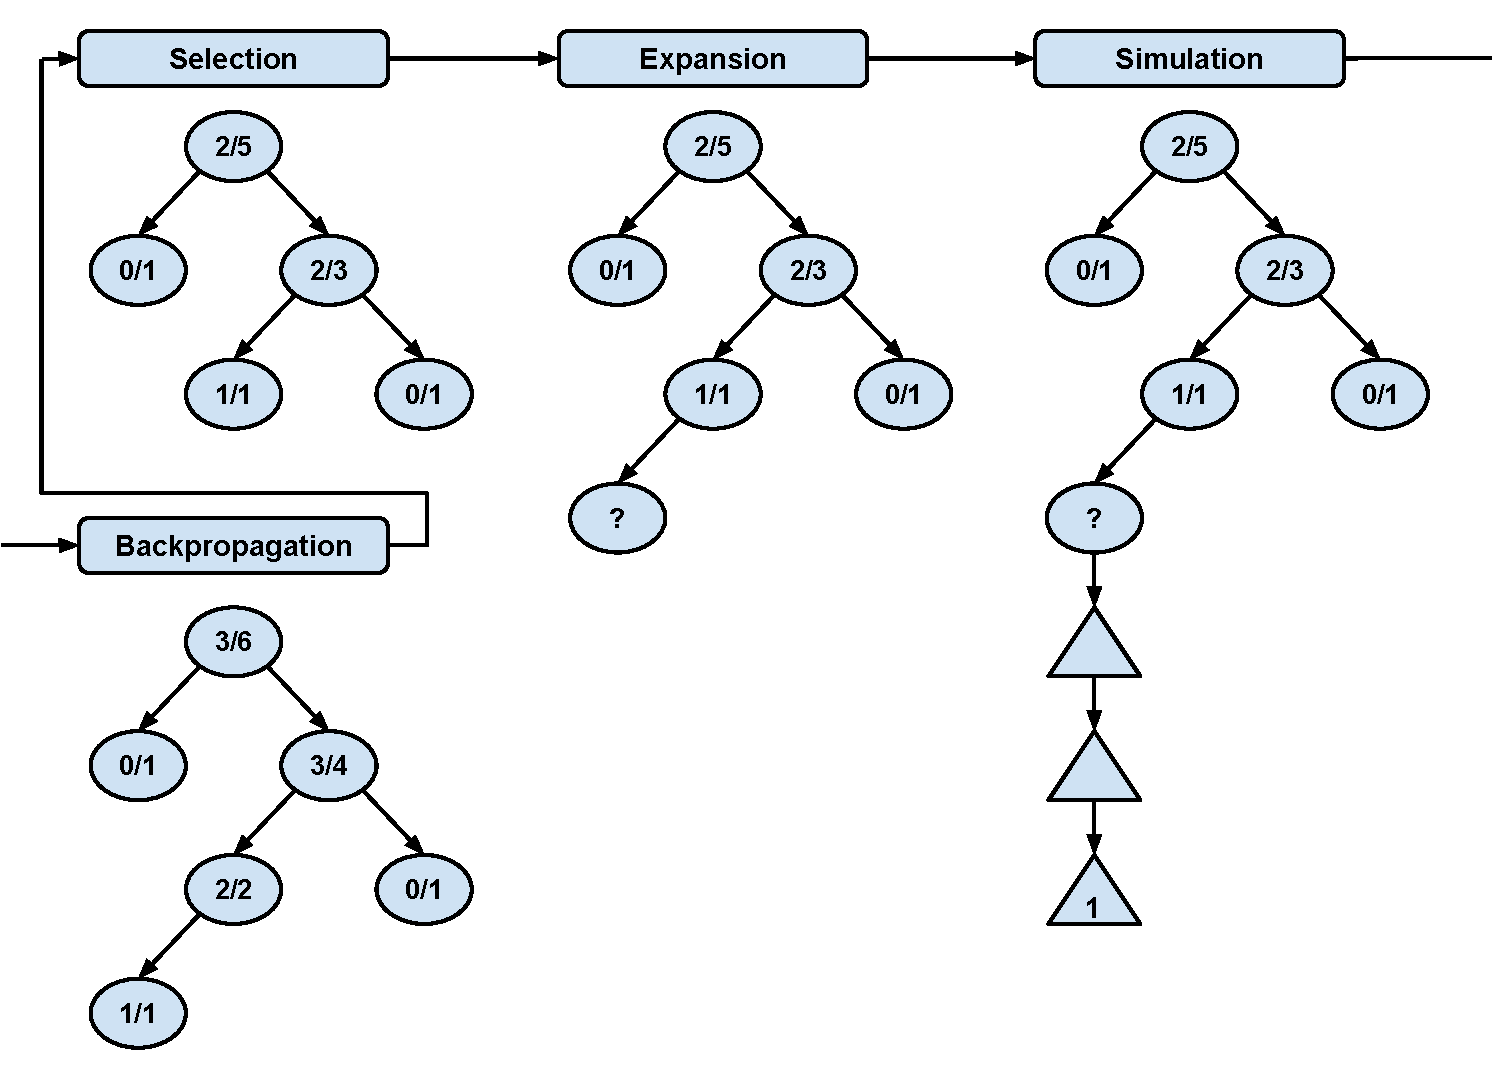
\includegraphics[width=8.5cm]{MCTSFourStepProcess.pdf}
	\centering
	\caption{The four steps of MCTS}
	\label{fig:FourSteps}
\end{figure}

\todo{This section still needs a lot of work}
\todo{Explain what the numbers represent earlier}

\textbf{Selection} - In the selection process, the MCTS algorithm traverses the current tree using a tree policy. A tree policy uses an evaluation function that prioritize nodes with the highest estimated value. In figure \ref{fig:FourSteps} the MCTS algorithm traverses to the 2/3 node then the 1/1 because those are the nodes with the greatest estimated value.

\textbf{Expansion} - In expansion a new node is added to the tree as a child of the node reached in the previous step. There is only one node added to the tree in each iteration, and it is at this step. In figure \ref{fig:FourSteps} the newly added node is indicated by the ?.

\textbf{Simulation} - In this step, a simulation(also referred to as a playout or rollout) is played out according to the simulation policy\cite{ActionSelection}. The simulation may use either a weak or strong policy. A weak policy would use little to no predetermined strategy. It would simply playout the simulation randomly. A strong policy would use a more guided approach to choose the moves. A strong policy may make the simulation too deterministic or make it more prone for error\cite{TheGrandChallenge}. The policy plays out moves until either an end state or a predefined threshold is reached. Then based on the result of the simulation, the value of the newly added node is established. For example, a simulation of a node for Go would reach the end of a game(the end state), and then determine a value based on whether the player won, or lost. In \ref{fig:FourSteps} the simulation ended in a 1. Therefore, the value of the new node is 1/1.

\textbf{Backpropagation} - Once the value of the node is determined, then as the name of this process implies, the rest of the tree can be updated. The algorithm will traverse back to the root node only updating the values of the nodes that it passes through. Only those nodes are effected because each node's respective value is an estimation of values of the nodes after them. In figure \ref{fig:FourSteps} there are two nodes that are left untouched since those do not branch into the newly added node.

\subsection{Upper Confidence Bound Applied to Trees(UCT)}
\todo{Get across that each unexplored node is explored before moving on, but only at each node that is visited. If a node is not visited again, that node's children will not be explored.}
The UCT is what the MCTS algorithm uses as a tree policy to traverse the tree. The goal of the UCT is to balance the idea of exploration versus exploitation. The concept of exploration promotes exploring many unexplored areas. This approach may explore many different paths on its way to finding the best decision. While this approach is useful to ensure that MCTS is not overlooking any potential paths, it can become very inefficient very quickly with games with a large number of moves. This is balanced with exploitation. The exploitation approach will tend to stick to one path that has the greatest estimated value. UCT balances these two ideas by exploring every unexplored node that it visits, but then it only visits nodes that yield the greatest estimated value.

 \begin{equation}
 \label{UCTequation}
 UCT(node) = \frac{W(node)}{N(node)} + \sqrt[c]{\frac{ln(N(parentNode))}{N(node)}}
 \end{equation}

When traversing the tree, Equation \ref{UCTequation} is applied to each of a node's children to evaluate the estimated value of that node\cite{ActionSelection}. N() represents the total number of simulations made at that node and the nodes branching off of it. W() represents how many of those simulations ended in a winning state. C represents an exploration constant that is found experimentally. The first part of the UCT takes into consideration the known estimated value of the node by determining the ratio of simulations won to total simulations. The second part of the UCT takes into consideration the unexplored nodes of the parent node by taking the ratio of the parent node's total simulations to the node's simulations.

\section{Using MCTS to play Go}
\todo{I could talk about a variation in their playout policy, but it would require a lot of explanation of Go, and I think it wouldn't add nearly enough to the paper to warrant the added explanation of Go.}
MCTS has seen a lot of success in its applications in Go. The computer Go programs MoGo and Crazy Stone both use MCTS, and they have had the best performance of any computer Go programs\cite{RAVEinGo}. Those programs use the traditional MCTS algorithm with the UCT approach, and they apply their own variations specifically in the context of Go.

\subsection{All Moves as First(AMAF)}
The all moves as first(AMAF) is a methodology that treats all moves as the next move to be made. That means that AMAF does not take into account the order in which moves are played. Moves have no context in this methodology. This methodology is quite useful when either moves played elsewhere do not have an effect on the value of a move, or if a game can arrive at the same state regardless of the order in which the moves are played.

\begin{figure}[h]
	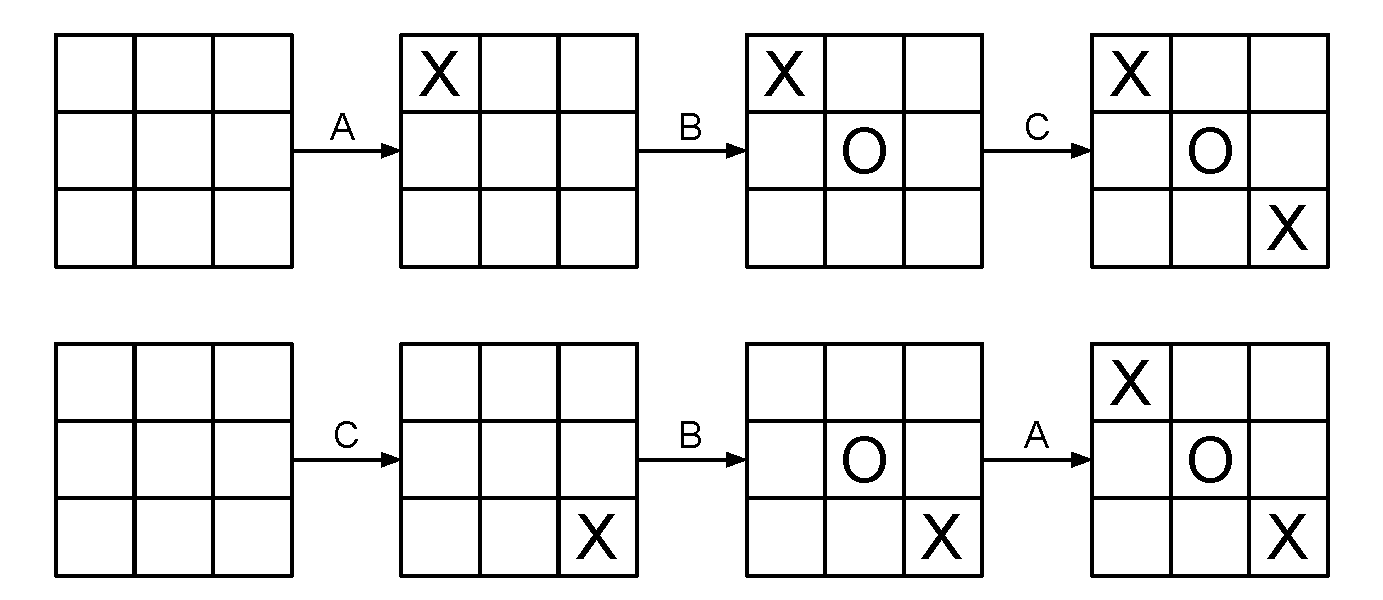
\includegraphics[width=8cm]{MoveOrderNotMattering.pdf}
	\centering
	\caption{Comparison of two sequences of moves in TicTacToe}
	\label{fig:TwoSeq}
\end{figure}

In figure \ref{fig:TwoSeq} are two possible sequences of moves that can be played out in the game TicTacToe. Even though the order in which moves A and C are played are different, it still results in the same game state. AMAF is useful in analyzing the effectiveness of this situation since the order in which the moves are played has no effect strategically. Thus, we can treat playing move A first or move C first as having the same strategic value.

The AMAF methodology is applicable to Go because many of the situations only affect what is happening locally. If a move is made elsewhere on the board, it does not have much of an affect on the strategic value of the move being examined. It is also important to note that in Go a move that repeats a board state is illegal. Therefore, this methodology will not have any inconsistencies with replaying the same move.

\subsection{Rapid Action Value Estimate}
Rapid action value estimate(RAVE) takes the concept of AMAF and stores the value of every move at every node in the tree. This means that each node contains the combined value of each move that has been played out in a simulation branching from that node. This is how the information must be stored for the MCTS algorithm to work because MCTS works on the assumption that each value that the node contains comes from the simulations performed at that node and the ones in the subtree of that node. This assumption must remain true since MCTS traverses the tree selecting for nodes with the greatest potential value.

\begin{figure}[h]
	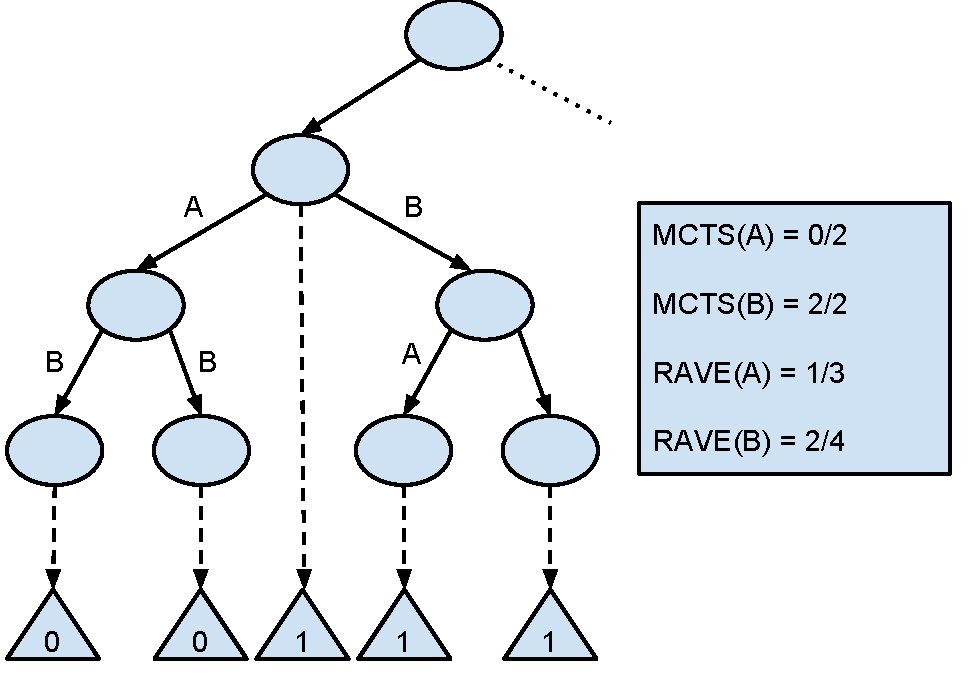
\includegraphics[width=8cm]{RAVEDiagram.pdf}
	\centering
	\caption{MCTS vs RAVE}
	\label{fig:RAVEDiagram}
\end{figure} 

The RAVE approach is very powerful and allows us to retrieve much more information out of every simulation that MCTS performs. Typically in MCTS only one piece of information would be gained by a simulation. That would be whether or not that specific node resulted in a win or a loss. Now, every move in that simulation provides the MCTS with information on the value of that move. This allows the MCTS algorithm to converge much more quickly on which move to perform next.

\subsection{MC RAVE}
The RAVE approach is very useful and efficient, but it can sometimes select an incorrect move\cite{RAVEinGo}. When the players have close tactical battles, the sequencing of the moves become very important. In this situation, we cannot treat the moves as AMAF. We still need the contextual dependencies of the MCTS approach.

MC RAVE combines the traditional MCTS algorithm and the RAVE approach into one algorithm. MC RAVE uses a weighted approach that combines the values from the MCTS value and the move values from RAVE. The weighted approach works as a sliding scale that gives more value to the MCTS value the more simulations that started from that node\cite{RAVEinGo}. Inversely, if only a few simulations have been played out, the RAVE value would have more weight.

The MC RAVE approach works because the strength of the RAVE approach is that it provides a lot of information and converges quickly with relatively few simulations. The MCTS approach is given more weight as more simulations are performed because it gives a much more accurate estimation of the contextual dependencies, but it requires more simulations than RAVE.

\subsection{Results}
Computer programs that used more traditional approaches to playing game have had very little success playing Go. The deterministic approaches struggled to defeat even low rank amateurs. Now with new Go programs implementing MCTS, they have achieved a lot of success and the achievements are only growing. The top computer programs can now compete with top professionals in 9x9 Go\cite{RAVEinGo}. Not only that, but those programs can even compete against the top pros in handicap games of 19x19 games of Go. That is an incredible feat taking into consideration the immense complexity of a 19x19 board. Clearly, MCTS has demonstrated its impact on AI approaches to Go.

\section{Using MCTS for Narrative Generation}
MCTS has demonstrated that it has applications outside of playing board games. Kartal et al\cite{Narrative} used MCTS to generate narratives. Their algorithm uses a list of actors, items, and places along with various actions that let those things interact with each other. The user then specifies the initial setup and overall goal for the story.

\subsection{Tree Representation}
As stated previously, the nodes of the MCTS tree represents the state of the system at that node. In narrative generation, the nodes will hold the information of what action is happening, and the current attributes of the actors. Any previous nodes will hold the information about the story that happened up to the current node's step in the narrative with the root node being the very first action taken in the narrative.

The attributes of the actors are simply information that is needed to help describe the story. An actor may have attributes that describe their name, their current health, their current location, or the  current anger level of the actor. Certain actions become more likely or less likely to occur depending on these attributes.

\begin{itemize}
\item \textbf{Move(A, P):} A moves to place P.
\item \textbf{Kill(A, B):} B's health to zero(dead).
\item \textbf{Earthquake(P):} An earthquake strikes at place P. This causes people at P to die (health=0), items to be stuck, and place P to collapse.
\end{itemize}

Here is a small sample of possible actions that may occur in a story. It would not make much sense if actor A killed actor B if actor B did not interact with actor A. Although if actor A's anger is sufficiently high, it may make it more believable for this action to occur\cite{Narrative}.

\subsection{Narrative Simulation}
\todo{I should make clear the two different heuristic methods they introduced, so it is easier to contrast them in the results}
In Go, the simulation step of MCTS would end in either a win or a loss, but that approach does not really apply to narrative generation. Instead the authors chose to establish a threshold for their simulation policy. When the story in the simulation reaches a certain length, or if the story accomplishes a predefined amount of the goals outlined by the user, the simulation will then stop and be evaluated.

To establish a value for the simulation, the authors developed a believability function. The believability function evaluates the simulation based on how believable the narrative is, and how many goals the narrative accomplished. The believability is based on the order in which the actions occur and how likely they are to occur given prior events.

The believability functions strikes a balance between goal completion and believability because it would not make for a good narrative without either. A narrative could easily complete the goals laid out by the user without being very believable, and a narrative could be very believable while not accomplishing any of the goals. Sometimes this results in one being sacrificed for the other. For example, maybe a long series of actions that are not the most believable are used for the sake of completing the goals of the narrative. While this outcome is not perfect, it is preferable over the two extremes.

In the simulation process the authors decided to use a guided approach. Their algorithm uses a table that keeps track of various actions that have occurred in the simulations and their respective average evaluation score. The algorithm uses these scores to bias the random sampling in the simulations in favor of actions that have produced higher evaluation scores in the past. 
\subsection{Tree Pruning}
The trees for MCTS can get very memory intensive, so the authors decided to implement tree pruning into their algorithm to essentially allow for the algorithm to use the memory it is allocated more efficiently. In tree pruning, an algorithm will selectively cut out pieces of the tree that do not seem very promising.  

The authors implemented tree pruning by only allowing the algorithm to plan out the narrative one step at a time. When the next step is being selected, the algorithm will run for a predefined number of iterations. After those iterations have been run, the algorithm will choose the node with the greatest potential value that is a child of the current root node. The chosen node effectively becomes the new root node of the tree while keeping track of the steps that preceded it. When the new node is chosen, all other children from the previous node are discarded. The memory that those nodes were allocated can now be used for future simulations. This process allows for the algorithm to much more efficiently use the memory it is allocated.

The authors do make note that this approach makes the algorithm no longer probabilistically complete. This means that it is possible that one of the branches that is pruned would be preferable to the current path. The current path may just be a local maxima instead of the preferred global optimum. Even with this flaw, the authors still found their algorithm to perform reasonably well. 

\subsection{Results}
The authors compared their results to three different tree search approaches: Breadth-First Search, Depth-First Search, and Best-First Search\cite{Narrative}. Each of these algorithms should provide the optimal solution if given enough time and memory. Depth-First Search and Best-First search in particular are capable of finding the solution very early on in the search.

They compared these four algorithms allowing them two different amounts of nodes. The first comparison allowed the algorithms up to 100 thousand nodes, and the second comparison allowed the algorithms up to 3 million nodes. They are then compared on the score each one achieved from the believability function.

In the first comparison, the only algorithm that came close to MCTS was the Breadth-First Search algorithm. Bread-First Search scored on average over three trials of .05, while the MCTS scored a .07. The other two algorithms scored below .01. When the algorithms were allocated 3 million nodes, MCTS far and away outperformed the other algorithms. MCTS scored .09 while the others didn't even get up to .01.

The authors compared their playout biasing approach to a MCTS algorithm without it. They found that given a low budget of nodes, the typical MCTS algorithm outperformed their biased approach. Alternatively, they found that when the algorithms were allowed a large number of nodes, the biased approach far outperformed the typical MCTS approach. The authors also compared their tree pruning approach to a typical MCTS algorithm. They found that the typical MCTS algorithm would quickly run out of memory when given a large number of actors, items, and places. The tree pruning approach used memory much more efficiently and found much higher scoring stories than the typical MCTS algorithm.

\section{Conclusions}

\section{Acknowledgements}

\section{References}

\subsection{Citations}

% The following two commands are all you need in the
% initial runs of your .tex file to
% produce the bibliography for the citations in your paper.
\bibliographystyle{abbrv}
% sample_paper.bib is the name of the BibTex file containing the
% bibliography entries. Note that you *don't* include the .bib ending here.
\bibliography{MaxMagnusonSeniorSeminar}  
% You must have a proper ".bib" file
%  and remember to run:
% latex bibtex latex latex
% to resolve all references

\end{document}
